\documentclass[10pt]{article}
\usepackage[T1]{fontenc}
\usepackage[utf8]{inputenc}
\usepackage{lmodern}
\usepackage[margin=0.7in]{geometry}
\usepackage{amsmath,amssymb}
\usepackage{microtype}
\usepackage{enumitem}
\usepackage{graphicx}
\usepackage{float}
\usepackage{booktabs,array}
\usepackage[font=small,labelfont=bf,skip=3pt]{caption}
\captionsetup[figure]{font=footnotesize}
\usepackage[dvipsnames]{xcolor}
\usepackage[backend=bibtex,style=authoryear,natbib=true,maxcitenames=2,maxbibnames=4,minbibnames=3,uniquelist=false,uniquename=false,giveninits=true,doi=false,isbn=false,url=false,eprint=false]{biblatex}
\addbibresource{smoothed_muon.bib}
\usepackage[colorlinks=true,linkcolor=MidnightBlue,citecolor=MidnightBlue,urlcolor=MidnightBlue]{hyperref}
\usepackage[capitalise,nameinlink]{cleveref}
\setlength{\parskip}{2pt}
\setlength{\parindent}{0pt}
\setlist{nosep,leftmargin=*}
\setlength{\textfloatsep}{8pt}
\setlength{\intextsep}{6pt}
\makeatletter
\renewcommand\paragraph{\@startsection{paragraph}{4}{\z@}{1.0ex \@plus .3ex \@minus .2ex}{-1em}{\normalfont\normalsize\bfseries}}
\renewcommand\maketitle{\begin{center}{\large\bfseries\@title\par}\vspace{3pt}\@author\quad\textperiodcentered\quad\@date\end{center}}
\makeatother

\title{Smoothed Muon Under the Cross-Entropy Loss\\[1pt]
\normalfont The CE report with a third optimizer, MIT 6.7910, Fall 2026}
\author{Juntang Wang and V\'ictor Conchello}
\date{November 2026}

\begin{document}
\maketitle
\vspace{-0.8em}

\paragraph{Summary.} Under the cross-entropy (CE) loss, as in our earlier study under the mean squared error (MSE,
\texttt{results/smoothed\_muon.pdf}), giving Muon AdamW's cosine between consecutive updates (0.88 instead of 0.74)
moves almost none of Muon's properties towards AdamW's. \emph{Smoothed Muon} is Muon with each step a running average
of Muon's orthogonalized updates; we set the averaging so that this cosine is AdamW's. We then add
smoothed Muon to our comparison of AdamW and Muon under CE (the \emph{CE report}, \texttt{checkpoint/checkpoint.pdf}),
on the same five data orders (mini-batch sequences). (1)~Speed, final loss and path (the sequence of next-token predictions over training) stay close to Muon's. The final
validation loss is 1.314 (Muon 1.309, AdamW 1.344). On the same mini-batches, smoothed Muon's predictions are closer
to Muon's (Jensen--Shannon divergence 0.049 at the end) than AdamW's are (0.058). (2)~Weight spectra and MLP sparsity
(the share of MLP units with a positive input) are Muon's. At equal training loss, no
prediction metric differs between any two optimizers by more than its spread over data orders. (3)~Besides the update
itself (9\% shorter than Muon's, and less aligned with the negative gradient), only the curvature differs from
Muon's by more than 5\%. From step 1500 on, the Hessian trace is 5 to 9\% below Muon's. The top Hessian eigenvalue is
above Muon's early in training (by 16\% at training loss 1.81) and 8 to 13\% below it from step 5000 on. (4)~In runs
that switch between AdamW and smoothed Muon mid-training, in either direction, the final weights depend on the
switching step as they do for switches between AdamW and Muon. Switches between Muon and smoothed Muon bring the
cosine to the new optimizer's level and move the curvature partly; the weight spectra and the share of active MLP
units stay as they are. Two results differ from MSE: at
Muon's learning rate, smoothed Muon ends slightly behind Muon (under MSE they tie), and its Hessian trace ends only 8\%
below Muon's (under MSE, 40\% below).

\paragraph{Setup.} \emph{Model and loss.} Everything is as in the CE report (\texttt{checkpoint/checkpoint.pdf}): a
14M-parameter nanoGPT \citep{karpathy2022nanogpt} on TinyStories \citep{eldan2023tinystories}, 10{,}000 steps of 128
sequences of 256 tokens, with the cross-entropy loss (settings: \cref{app:hparams}).

\emph{Muon.} Muon \citep{jordan2024muon} updates each weight matrix $W$ of the transformer blocks separately; AdamW
trains the other parameters (embeddings, output head, LayerNorm gains). With $G_t$ the gradient of $W$ at step $t$,
$\beta=0.95$ and learning rate $\eta$,
\[
M_t=\beta M_{t-1}+(1-\beta)G_t,\qquad N_t=(1-\beta)G_t+\beta M_t,\qquad O_t=\operatorname{msign}(N_t),\qquad
W_t=W_{t-1}-\eta\,O_t .
\]
$M_t$ is a momentum, $N_t$ its Nesterov form, and $\operatorname{msign}$ \emph{orthogonalizes}: it sets every singular
value of $N_t$ to about 1.

\emph{Smoothed Muon.} Only the last formula changes: the step follows a running average $U_t$ of the $O_t$,
\[
U_t=(1-a)\,U_{t-1}+a\,O_t,\qquad W_t=W_{t-1}-\eta\,\frac{U_t}{1-(1-a)^t},\qquad U_0=0 .
\]
The division keeps the first steps at full size. With $a=1$ this is Muon. A smaller $a$ spreads each $O_t$ over the
following steps: a share $a$ of it is applied at step $t$, $a(1-a)$ at step $t+1$, and so on.

\emph{Choosing $a$ and $\eta$.} We measure how alike consecutive updates are by their cosine
$\cos(\Delta\theta_t,\Delta\theta_{t+1})$, where $\Delta\theta_t=\theta_{t+1}-\theta_t$ is the step of all parameters.
We compare optimizers at training loss 1.81, as the CE report does: AdamW reaches it near step 1450 and Muon near
step 860. There the cosine is 0.88 for AdamW and 0.74 for Muon. Short runs of smoothed Muon (to step 2000, at Muon's
$\eta=0.01$) show that a smaller $a$ raises it (\cref{tab:calib}). We take $a=0.65$: its cosine is the closest to
AdamW's at that loss (0.883 against 0.881, on data order 0). Smoothed Muon keeps Muon's learning rate, $\eta=0.01$, so that it differs
from Muon in the averaging alone (\cref{app:calib} gives a learning-rate sweep). It then runs from the same
initialization and on the same five \emph{data orders} (mini-batch sequences) as AdamW and Muon.

\begin{table}[H]
\centering\small
\caption{Choosing $a$: cosine between consecutive updates at training loss 1.81 and validation loss at step 2000,
on data order 0 with $\eta=0.01$. AdamW: its full run on data order 0, at its own $\eta=2\cdot10^{-3}$. Second row: the
cosine over the 36 weight matrices of the transformer blocks only. Bold: the chosen $a$.}
\label{tab:calib}
\begin{tabular}{@{}l|c|ccccccc|c@{}}
 & Muon & \multicolumn{7}{c|}{smoothed Muon, $a=$} & AdamW \\
 & ($a=1$) & 0.8 & 0.7 & \textbf{0.65} & 0.6 & 0.55 & 0.5 & 0.4 & \\
\hline
Cosine at training loss 1.81 & 0.740 & 0.835 & 0.869 & \textbf{0.883} & 0.896 & 0.908 & 0.920 & 0.937 & 0.881 \\
Same, block matrices only & 0.690 & 0.812 & 0.857 & \textbf{0.877} & 0.894 & 0.911 & 0.927 & 0.951 & 0.876 \\
Validation loss at step 2000 & 1.588 & 1.598 & 1.595 & \textbf{1.596} & 1.599 & 1.596 & 1.606 & 1.613 & 1.696 \\
\hline
\end{tabular}

\end{table}

\paragraph{Step 1: how the trajectories differ (\cref{fig:div}).} \emph{Comparing runs.} The distance between two runs
is the mean Jensen--Shannon divergence (JS, in bits) of their next-token predictions on held-out text. We compare runs
at equal step and at equal training loss; at equal loss, speed does not count as a difference. The \emph{floor} of an
optimizer is the mean distance between its runs on two different data orders, over all 10 pairs of its five data
orders. Because it compares different mini-batches, it can
exceed the distance between two optimizers on the same data order.

\begin{figure}[H]
\centering
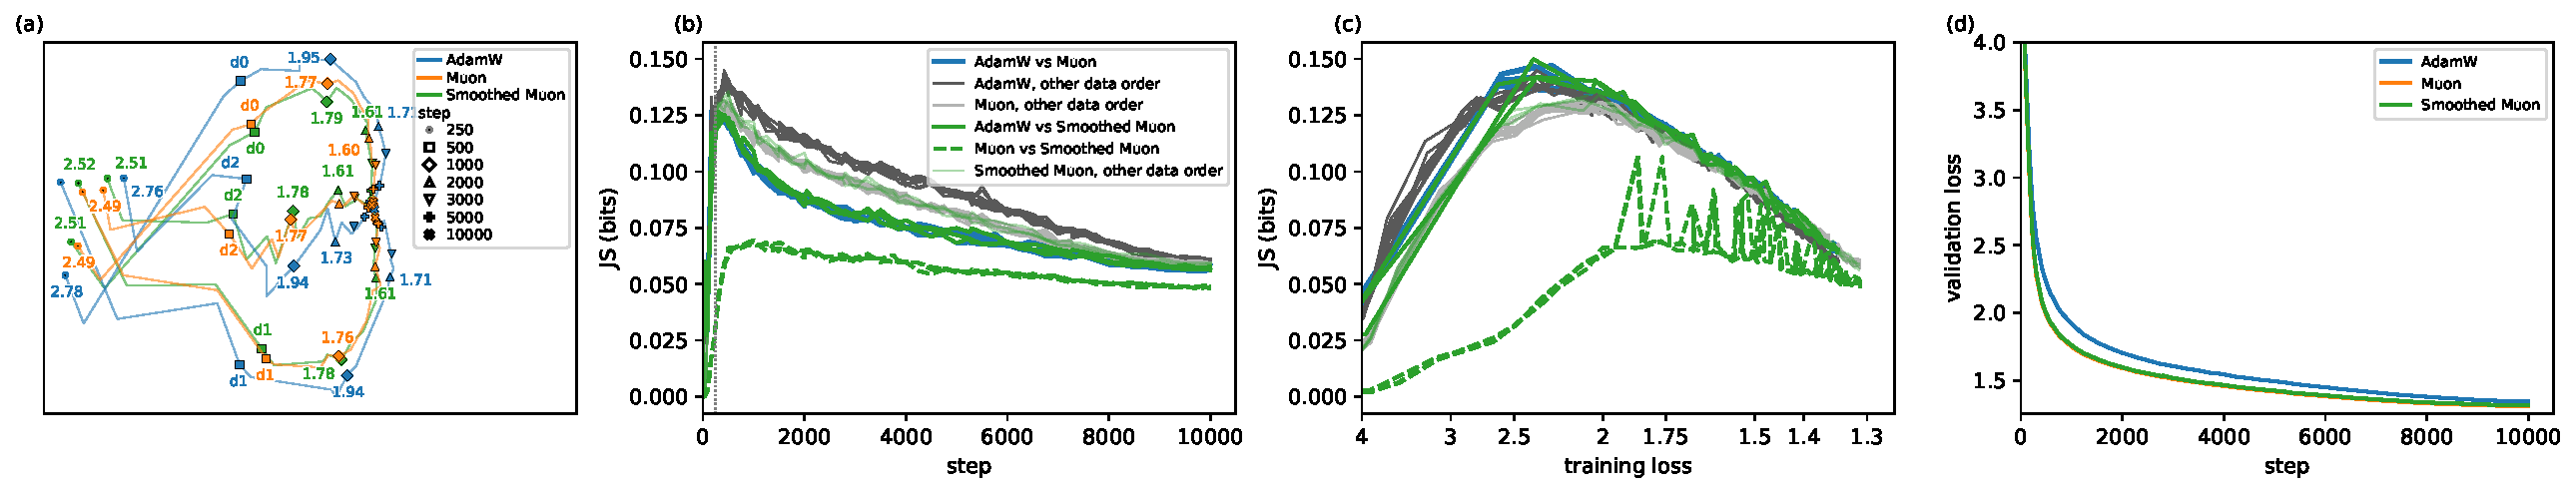
\includegraphics[width=\linewidth]{ts10m_smooth/divergence_umap.pdf}
\caption{AdamW, Muon and smoothed Muon. (a) Next-token predictions of the saved models of data orders 0--2 from step 250 on, mapped to 2-D
by densMAP (a variant of UMAP; shows neighbours, not distances); markers: step; labels: training loss and data
order. (b) JS between runs at equal step.
Blue: AdamW against Muon. Thick green: smoothed Muon against AdamW (solid) and against Muon (dashed), on the same data
order. Grey (AdamW, Muon) and thin green (smoothed Muon): one optimizer on two data orders, one line per pair; a floor is
the mean of an optimizer's 10 lines. Dotted line: step 250, where (a) starts. (c) The
same at equal training loss. (d) Validation loss; bands: range over data orders.}
\label{fig:div}
\end{figure}

\emph{Speed and endpoints: close to Muon's.} AdamW's final validation loss (1.344) is reached at step 7750 by
smoothed Muon, at step 7500 by Muon and at step 10{,}000 by AdamW itself (d). The final validation loss is 1.314 for smoothed Muon (1.310 to
1.318 over the five data orders), 1.309 for Muon (1.305 to 1.314) and 1.344 for AdamW (1.339 to 1.350). Smoothed Muon
is behind Muon on each data order, by 0.001 to 0.010: on average a seventh of the way from Muon to AdamW. Part of this
gap comes from the learning rate. On data order 0, smoothed Muon's best of five rates, $\eta=0.005$, ends at 1.309,
against 1.315 at $\eta=0.01$ and 1.305 for Muon (\cref{app:calib}).

\emph{Path: Muon's.} On the same data order, smoothed Muon stays closer to Muon than AdamW does, throughout training
(b): 0.056 against 0.071 at step 5000, and 0.049 against 0.058 at the end. Its distance to AdamW
(0.072 at step 5000, 0.057 at the end) equals Muon's (0.071, 0.058). The floors of the three optimizers are 0.081 to 0.090 at step 5000 and
0.058 to 0.060 at the end. At equal training loss (c) the picture is the same: at loss 2.0, smoothed Muon and Muon are
0.065 apart, while AdamW is 0.134 from Muon and 0.136 from smoothed Muon; the floors are 0.128 to 0.131. Below loss 2
the dashed curves in (c) spike. Models are saved every 250 steps and the training loss is noisy, so when two equally fast
runs are matched by loss, one run's model is sometimes matched to the other's model from 250 steps earlier or later.
That step offset, not a real difference, causes the spikes. In (a), each smoothed-Muon run lies next to the Muon run of its data order.

\paragraph{Step 2: what differs along the way.} We measure the 30 properties of the CE report at 34 points of
training, in five groups (\cref{app:metrics} defines them; \cref{tab:app-am,tab:app-sgd} give all values at training
loss 1.81, and \cref{tab:app-curv} the curvature over training). \Cref{fig:rank} shows two ratios at training loss
1.81, for the nine metrics of the CE report's ranking figure: AdamW/Muon and
smoothed Muon/Muon, on data orders 0--2. A green point at 1 means ``as Muon''; a green point on the black one means
``as AdamW''.

\begin{figure}[H]
\centering
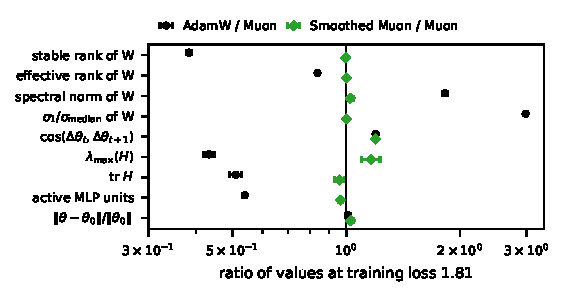
\includegraphics{ts10m_smooth/ranking.pdf}
\caption{Ratios to Muon at training loss 1.81, for selected metrics; three data orders each; bars: range across data
orders. Smoothed Muon's $\lambda_{\max}$ ratio (1.16) is above 1 because its high initial curvature decays more slowly;
from step 5000 on its $\lambda_{\max}$ is 8 to 13\% below Muon's (\cref{tab:app-curv}).}
\label{fig:rank}
\end{figure}

Smoothed Muon reaches training loss 1.81 near step 900. Values below are means over data orders 0--2 at
that loss, with Muon's and AdamW's in parentheses, unless a step is given.

\begin{itemize}
\item \emph{Weights $W$: Muon's.} The stable rank is 85.9 (Muon 86.2, AdamW 33.0), the effective rank 324 (325, 272),
the spectral norm 3.03 (2.95, 5.39) and $\sigma_1/\sigma_{\rm median}$ 2.68 (2.68, 8.01). The distance from the initialization
is 2.2 times the initial norm (2.2, 2.2). At the end of training the stable rank is still Muon's: 75 (75, 41).
\item \emph{One-step updates $\Delta\theta$.} The cosine between consecutive steps is AdamW's, as chosen: 0.883
(0.738, 0.883). It stays close to AdamW's: at step 9000 it is 0.888 (0.758, 0.898). The stable rank of $\Delta W$ is
Muon's, 219 (220, 17). The step is 9\% shorter than under the other two: $\|\Delta\theta\|/\|\theta\|$ is
$5.96\cdot10^{-3}$ ($6.53\cdot10^{-3}$, $6.56\cdot10^{-3}$). It also points less along the negative gradient: their
cosine is 0.157 (0.217, 0.244).
\item \emph{Loss curvature (Hessian $H$; \cref{tab:app-curv}).} Every run starts with a phase of high curvature, which
lasts longer under smoothed Muon. Its top Hessian eigenvalue $\lambda_{\max}$ falls below 20 by step 500, Muon's by
step 300. So at loss 1.81 its $\lambda_{\max}$, 16.6, is above Muon's (14.3) and even farther from AdamW's (6.2). From step 5000
on, it is 8 to 13\% below Muon's, and the ranges over data orders separate: at the end it is 20.0 (22.1, 8.7). The
trace $\operatorname{tr}H$ is below Muon's from step 500 on, with separate ranges: by 5\% at loss 1.81, where it is
2640 (2770, 1400), and by 5 to 9\% from step 1500 on. AdamW's trace is far below Muon's in mid-training (1070 against
1420 at step 4000), then climbs back towards Muon's. So from step 8000 on, the ranges of smoothed Muon and AdamW
overlap: at the end the trace is 1825 (1991, 1880).
\item \emph{Internal activations: Muon's.} 21\% of the MLP units are active, that is, have a positive input (22\%,
12\%). The attention entropy is 2.78 nats (2.79, 2.51).
\item \emph{Predictions: no differences.} For every prediction metric, the ranges of the ratios smoothed Muon/Muon
and AdamW/Muon contain 1 (\cref{tab:app-am}).
\end{itemize}

\paragraph{Step 3: swaps (\cref{fig:swap}).} \emph{Swaps.} A \emph{swap} switches a run of one optimizer (the
\emph{parent}, on data order 0) to another optimizer at a \emph{fork step}, then trains it to step 10{,}000 on the
parent's batches (\cref{app:forks}). An optimizer's \emph{own run} is its run from the start. We swap at nine fork steps
from 50 to 4000, in both directions, between smoothed Muon and each of AdamW and Muon: 36 swaps, next to the 18 between
AdamW and Muon of the CE report. The \emph{fraction} of a swap for one metric is
$(x_{\rm swap}-x_{\rm parent})/(x_{\rm new}-x_{\rm parent})$, all at step 10{,}000: 0 means the swap ends like the
parent's own run, 1 like the new optimizer's.

\begin{figure}[H]
\centering
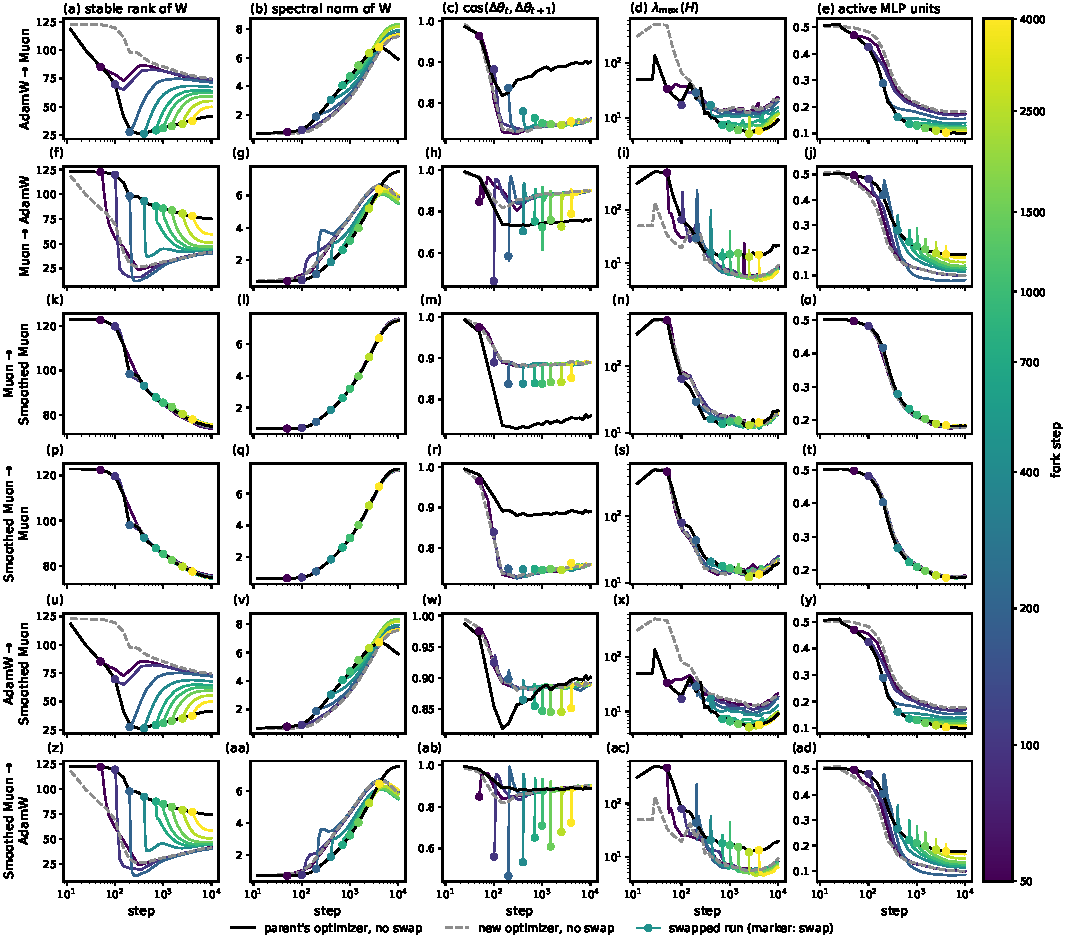
\includegraphics[width=\linewidth]{ts10m_smooth/swap_traj.pdf}
\caption{Swaps on data order 0: five metrics against the step, one row per direction. Black: the parent's optimizer
without a swap; grey dashed: the new optimizer's own run; colour: swapped runs, by fork step (dot: the swap).}
\label{fig:swap}
\end{figure}

\emph{In swaps with AdamW, smoothed Muon behaves as Muon (u--ad against a--j).} The earlier a swap from AdamW to smoothed
Muon, the closer its stable rank of $W$ ends to smoothed Muon's own run: fractions 0.94 at fork step 50, 0.79 at 400
and 0.26 at 4000 (to Muon: 0.94, 0.77 and 0.25). Swaps from smoothed Muon to AdamW end at AdamW's stable rank up to
fork step 200 (fractions 0.99 to 1.03) and about half-way at fork step 4000 (0.48, against 0.46 for the swap from Muon to AdamW).
For the stable rank and the share of active MLP units, at every fork step and in both directions, each
AdamW--smoothed-Muon swap's fraction is within 0.05 of the matching AdamW--Muon swap's. One difference: after a swap
from AdamW at fork step 700 or later, $\lambda_{\max}$ stays near AdamW's level under smoothed Muon (fractions $-0.06$
to 0.08), and below the swap to Muon at the same fork step every time (0.02 to 0.30).

\emph{Between Muon and smoothed Muon, the weights and MLP stay; the cosine moves fully and the curvature partly
(k--t).} The own runs of the two end with nearly the same weights and MLP (stable rank 75.0 for Muon and 74.7 for
smoothed Muon; 18.2\% and 17.8\% of MLP units active), and so do all 18 swaps (stable
rank 74.0 to 75.9; 17.7\% to 18.4\% active). The cosine between consecutive updates ends at the new optimizer's level
in all 18: 0.889 to 0.891 after a switch to smoothed Muon, and 0.759 to 0.760 after a switch to Muon (own runs:
smoothed Muon 0.890, Muon 0.761). The curvature of the two own runs differs by about 10\% on this data order
($\lambda_{\max}$ 21.6 for Muon and 19.6 for smoothed Muon, $\operatorname{tr}H$ 1989 and 1777), and the swaps mostly end on the new optimizer's side. After a switch to smoothed
Muon, $\lambda_{\max}$ ends at 18.9 to 20.0 and $\operatorname{tr}H$ at 1747 to 1844; after a switch to Muon,
$\lambda_{\max}$ ends at 21.5 to 24.9 and $\operatorname{tr}H$ at 1842 to 1998 ($\operatorname{tr}H$:
\cref{tab:app-swaptrace}).

\paragraph{Next steps.} (i)~Under both losses, giving Muon AdamW's cosine by averaging leaves Muon's speed, path,
weight spectra and MLP sparsity in place, and does not change how Muon swaps with AdamW. So the cosine between
consecutive updates does not explain these differences between AdamW and Muon; the orthogonalization itself is one
candidate. (ii)~Find why smoothing lowers the final Hessian trace by 40\% under MSE but by only 8\% under CE.

\clearpage
\printbibliography

\clearpage
\appendix
%% Appendix of smoothed_muon_ce.tex, \input right after \appendix.
\crefalias{section}{appendix}\crefalias{subsection}{appendix}
\section{Hyperparameters}
\label{app:hparams}

\begin{center}\small
\captionsetup{type=table}
\caption{Hyperparameters shared by the AdamW, Muon and smoothed-Muon runs.}
\label{tab:app-shared}
\begin{tabular}{@{}lp{0.74\linewidth}@{}}
\hline
Runs & AdamW and Muon $\times$ data orders d0--d4, smoothed Muon $\times$ d0--d2 (13). The AdamW and Muon runs are those of the CE
  checkpoint. As there, Step 2 uses a second set of AdamW and Muon runs on d0--d2, identical but for the saved
  checkpoints (\cref{app:metrics}); the smoothed-Muon runs serve both steps \\
\hline
Model & nanoGPT, pre-LayerNorm blocks \\
Layers, heads, width & 6, 6, 384 \\
MLP & GELU, width 1536 \\
Biases, dropout & none, none \\
Output head & untied \\
Attention projections & separate query, key, value \\
Context & 256 tokens \\
Parameters & 13.9M (10.6M without token and position embeddings and head) \\
\hline
Data & TinyStories (GPT-4 version) \\
Tokenizer & byte-level BPE, 4096 tokens, trained on the training split \\
Batch & 128 windows $\times$ 256 tokens \\
Window offsets & from the training split; generator seeded with (data order, step), same for every optimizer \\
\hline
Loss & cross-entropy of the next token \\
Steps & 10{,}000 \\
Tokens & 328M (about 0.6 epochs) \\
Learning rate & $\eta\,\varphi(t)$ at step $t$, every parameter group \\
Warmup & linear, $\varphi(t)=(t+1)/200$ for $t<200$ \\
Decay & cosine to $\varphi=0.1$ at step 10{,}000 \\
Gradient clipping & none \\
\hline
Initialization seed & 0, all runs \\
Training precision & bfloat16 autocast \\
Prediction, Hessian precision & float32, no autocast (TF32 matrix products allowed) \\
\hline
Logged predictions & next-token distributions: 128 fixed validation sequences $\times$ 16 evenly spaced positions
  (2{,}048), as float16 log-probabilities \\
Training loss & 64 fixed training sequences, all positions; used to match runs at equal loss \\
Floor & mean JS between two data orders of one optimizer, at equal step or equal training loss \\
Both logged at & every 250th step $+$ 30 log-spaced steps in $[1, 10{,}000]$ \\
\hline
Hessian & top eigenvalue, 20 Lanczos iterations, 32 fixed training sequences \\
Measured at & every 500th step $+$ 30 log-spaced steps \\
\hline
\end{tabular}
\end{center}

\begin{center}\small
\captionsetup{type=table}
\caption{Optimizer-specific hyperparameters. $n_{\rm out}$, $n_{\rm in}$: output and input size of the matrix.
Smoothed Muon differs from Muon in the rows ``Step'' and $\eta$ only.}
\label{tab:app-optim}
\setlength{\tabcolsep}{4pt}
\begin{tabular}{@{}p{0.15\linewidth}p{0.25\linewidth}p{0.27\linewidth}p{0.27\linewidth}@{}}
\hline
 & AdamW & Muon & Smoothed Muon \tabularnewline
\hline
$\eta$ & $2\cdot10^{-3}$ & 0.01 & 0.01 \tabularnewline
$\eta$ choice & \raggedright best final validation loss of a 5-rate sweep on d0 & as AdamW &
  Muon's \tabularnewline
Update $O_t$ & bias-corrected moments & \raggedright Nesterov momentum; 5 quintic Newton--Schulz steps in bfloat16 &
  as Muon \tabularnewline
Step & $-\eta\,O_t$ & $-\eta\,O_t$ & \raggedright $-\eta\,U_t/(1-(1-a)^t)$, $U_t=(1-a)U_{t-1}+aO_t$, $a=0.65$
  \tabularnewline
Momentum & $\beta=(0.9,0.95)$ & $\beta=0.95$ & as Muon \tabularnewline
$\epsilon$ & $10^{-8}$ & -- & -- \tabularnewline
Update scale & -- & $\sqrt{\max(1,n_{\rm out}/n_{\rm in})}$ & as Muon \tabularnewline
Weight decay & \raggedright 0.1, decoupled; none on LayerNorm gains & none & none \tabularnewline
Parameters & all & \raggedright query, key, value, attention-output and both MLP matrices of every block & as Muon
  \tabularnewline
\hline
Aux.\ AdamW & -- & embeddings, head, LayerNorm gains & as Muon \tabularnewline
Aux.\ $\eta$, $\beta$, $\epsilon$ & -- & $2\cdot10^{-3}$, $(0.9,0.95)$, $10^{-8}$ & as Muon \tabularnewline
Aux.\ weight decay & -- & none & none \tabularnewline
\hline
\end{tabular}
\end{center}

\section{Calibration of smoothed Muon}
\label{app:calib}

We chose $a$ from short runs on data order 0 at Muon's learning rate, $\eta=0.01$: as in \cref{tab:app-shared}, but
without Hessian measurements and stopped at step 2002 (the learning-rate schedule is that of 10{,}000 steps). The cosine
between consecutive updates, $\cos(\Delta\theta_t,\Delta\theta_{t+1})$ with $\Delta\theta_t=\theta_{t+1}-\theta_t$,
comes from checkpoints at $t,t+1,t+2$, for eight values of $t$ from 400 to 2000. \Cref{tab:calib} gives it at training
loss 1.81, interpolated between the checkpoints at steps 800 and 1000, where every short run passes that loss. It barely
changes over these steps: for each $a<1$, its eight values lie within 0.008 of each other (Muon: 0.731 to 0.749).

\Cref{tab:calib} also gives the cosine for the 36 weight matrices of the blocks alone. These are the only parameters
whose update rule differs between Muon and smoothed Muon; AdamW trains the others under all three optimizers. With
$a=0.65$ the block matrices also match AdamW (0.877 against 0.876). The run with $a=1$ repeats Muon's run exactly: its
validation loss at step 2000 is Muon's, 1.5878.


\end{document}
